\chapter{Aplicación multimedia}
\section{Enunciado}
Las aplicaciones multimedia en tiempo real permiten conectar a distintos usuarios a través de la red e intercambiando información de audio,vídeo u otro tipo. Un ejemplo de este tipo de aplicación es Skype que ha tenido mucho éxito ya que permite a sus usuarios establecer videollamadas e intercambiar información una vez se haya instalado el software.
\begin{figure}[!h]
\begin{center}
   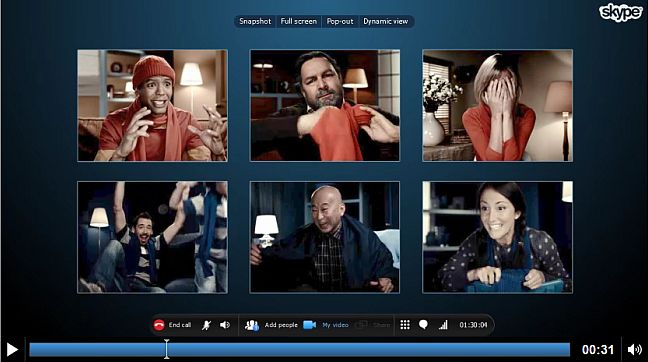
\includegraphics[width=0.9\linewidth]{Figures/skype}
	\decoRule
	\caption[Ejemplo sitio Web]{Skype interfaz videollamada.}
\label{fig:canvasPrimitivas}
\end{center}
\end{figure}
\\Por lo tanto en esta ultima practica se pide desarrollar una aplicación web similar a Skype que permita a los usuarios conectarse entre si a través de la url de la aplicación.Una vez dentro el usuario selecciona los elementos multimedia(audio y video) que desea compartir y tendrá que elegir si unirse o crear una sala donde los usuario mantendrán la comunicación.
\\Por ultimo, se podrá enviar cadena de texto entre los usuarios de una determinada sala a través del chat de la aplicación al igual que enviar archivos.
\subsection{Tecnologías necesarias}
\begin{enumerate}
\item API WebRTC
\item API File
\item NodeJS
\item Socket.io
\item JavaScript
\item Boostrap
\end{enumerate}
\subsection{Objetivos}
La practica tiene que cubrir los siguientes puntos
\begin{enumerate}
\item Creación/Unión de salas por parte de los usuarios.
\item El usuario seleccionara los elementos multimedia a compartir.
\item Transmisión de los elementos multimedia seleccionados entre los usuarios.
\item Creación de un servidor de señalizacion.
\item Topologia de comunicación en Malla.
\item Comunicación final Peer-to-Peer entre los navegadores.
\end{enumerate}
\section{Desarrollo}
Las próximas secciones trata la funcionalidad del cliente y servidor para entender mejor las funciones de cada uno.
%%%%%%%% Servidor Desarrollo %%%%%%%%
\section{Servidor de señalización}
El primer paso para crear el servidor es importar la librería \textbf{node-static},\textbf{http} y \textbf{socket.io}. La librería \textbf{http} permite crear un servidor a través del método \textbf{createServer} en el puerto 8181 en nuestro caso mientras que la librería \textbf{node-static} permite enviar el documento a los usuarios que se conecten.
\\Finalmente, la librería \textbf{socket.io} se utiliza para establecer comunicación entre el cliente y servidor, figura \ref{fig:EjecucionServer}.
\begin{lstlisting}[
caption=Creación Servidor de Señalizacion.]
 var static = require('node-static');
 var http = require('http');
 var file = new(static.Server)();
 var app = http.createServer(function (req, res) {
  file.serve(req, res);
 }).listen(8181);
 var io = require('socket.io').listen(app);
\end{lstlisting}
\begin{figure}[!h]
\begin{center}
   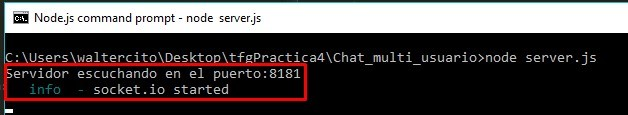
\includegraphics[width=0.8\linewidth]{Figures/InicioServidor}
	\decoRule
	\caption[ServidorSeñalizacion]{Ejecución Servidor de Señalizacion APP.}
\label{fig:EjecucionServer}
\end{center}
\end{figure}
El siguiente paso es permitir al servidor gestionar adecuadamente cada conexión que se establece a través de socket.io.Por ello, a través del método 'conected' mantendremos conectado.
\\Primero se define el evento \textbf{InfoRoom} que gestiona las peticiones sobre las salas disponibles.A esta petición el servidor contesta con un mensaje \textbf{ReplayInfoRoom} con la lista de las salas en la variable \textbf{listRoom}, figura \ref{fig:EjecucionInfoRoom}.
\begin{lstlisting}[,
caption=Request/Replay lista de salas existentes.]
 socket.on('infoRoom',function(name) {
  socket.emit('ReplayInfoRoom',listRooom);
 });
\end{lstlisting}
\begin{figure}[!h]
\begin{center}
   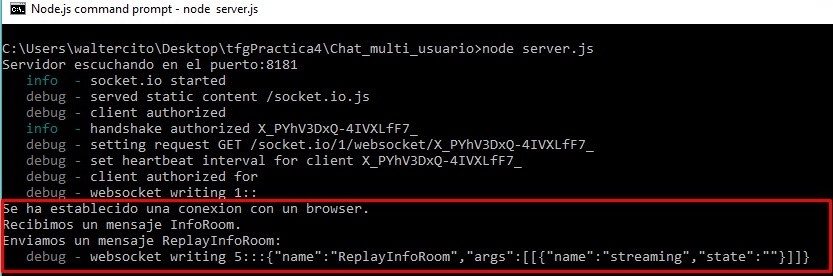
\includegraphics[width=0.8\linewidth]{Figures/InfoRoomServer}
	\decoRule
	\caption[Request/Replay Salas Servidor]{Request/Replay lista de salas del Servidor.}
\label{fig:EjecucionInfoRoom}
\end{center}
\end{figure}
Tras el envió de la lista de salas disponibles el servidor recibirá un mensaje ..Definimos el evento \textbf{Stablish\_connect} que recibe el nombre y sala a la que el usuario desea conectarse. Con esta información comprueba si el nombre de sala existe a través de la función \textbf{getRoom(nameRoom)} en caso de no existir se guardara en la lista con la función \textbf{setRoom()}.
\\Ademas, comprueba que la sala no este completa para enviar un mensaje \textbf{CreateStream} con el identificador de conexión y un mensaje  \textbf{NewJoined} al resto de usuario de la sala para que conozcan la existencia del nuevo miembro, figura \ref{fig:EjecucionStablishConnection}.
\begin{lstlisting}[
caption=Request/Replay del establecimiento de conexion.]
 socket.on('stablish_connection',function(name,room){
  if(!getRoom(room)){
    setRoom(room,'');
  };
  var numClients = io.sockets.clients(room).length;
  if(numClients < 3){
   socket.username = name;
   socket.room =room;
   socket.join(room);
   socket.emit('CreateStream',socket.id);
   socket.broadcast.to(room).emit('New_Joined',socket.id);
  }else{
   socket.emit('RejectStream',socket.id);
  }
 });
\end{lstlisting}
\begin{figure}[!h]
\begin{center}
   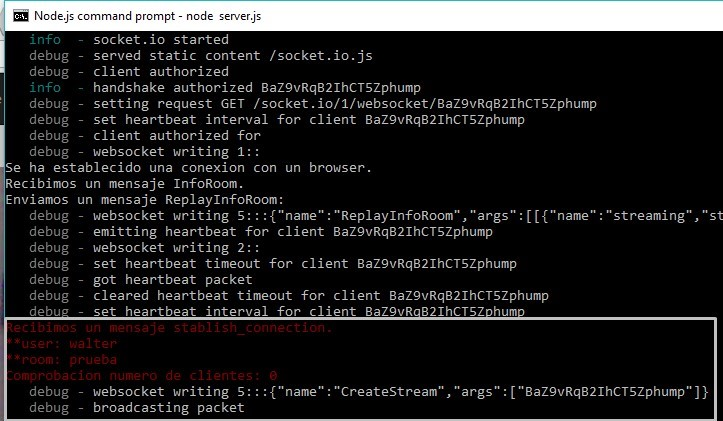
\includegraphics[width=0.8\linewidth]{Figures/StablishConnectionServer}
	\decoRule
	\caption[Request/Replay conexión Servidor]{Request/Replay conexión al Servidor.}
\label{fig:EjecucionStablishConnection}
\end{center}
\end{figure}
Tras haber enviado el mensaje \textbf{New\_Joined} definimos el evento \textbf{message} para gestionar los mensajes de señalizacion entre navegadores ya que el servidor es transparente a este proceso.
\begin{lstlisting}[
caption=Mensajes de señalizacion.]
 socket.on('message',function(message,room){
  io.sockets.socket(message.id_dest).emit('message', message);
 });
\end{lstlisting}
La figura \ref{fig:AnswerServer} encamina la oferta, la figura \ref{fig:OfferServer} encamina la oferta y la figura \ref{fig:IceCandidateVideos} encamina los IceCandidate.
\begin{figure}[!h]
\begin{center}
   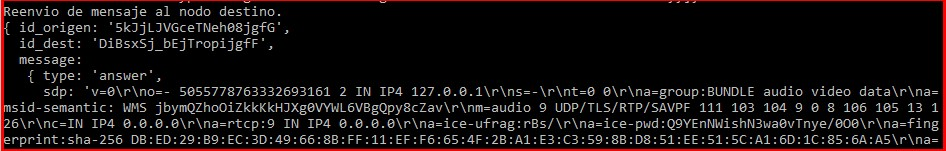
\includegraphics[width=0.8\linewidth]{Figures/AnswerServer}
	\decoRule
	\caption[Request/Replay conexión Servidor]{Mensaje tipo Answer.}
\label{fig:AnswerServer}
\end{center}
\end{figure}
\begin{figure}[!h]
\begin{center}
   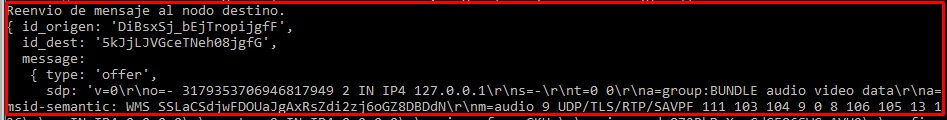
\includegraphics[width=0.8\linewidth]{Figures/OfferServer}
	\decoRule
	\caption[Request/Replay conexión Servidor]{Mensaje tipo Offer.}
\label{fig:OfferServer}
\end{center}
\end{figure}
\begin{figure}[!h]
\begin{center}
   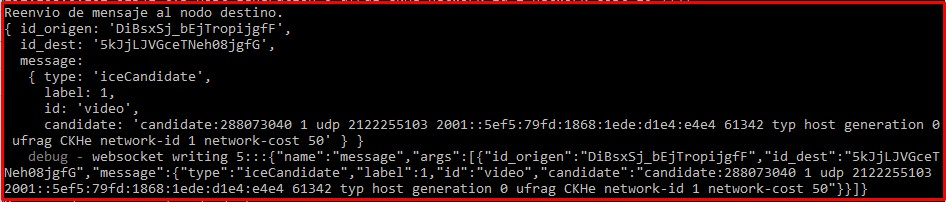
\includegraphics[width=0.8\linewidth]{Figures/IceCandidateVideos}
	\decoRule
	\caption[Request/Replay conexión Servidor]{Mensaje tipo Icecandidate.}
\label{fig:IceCandidateVideos}
\end{center}
\end{figure}
El servidor deja de participar en el intercambio de información entre los peers cuando el proceso de señalizacion termina ya que desde ese momento la comunicación es Peer-to-Peer.
%%%%%%%% Cliente Desarrollo %%%%%%%%
\section{Cliente}
Los usuarios se conectan al servidor a través de la url \textbf{http://localhost:8181} en un navegador que recibe el fichero \textbf{index.html}\footnote{Apéndice 4: Index}.
\\Se establece la conexión con el servidor a través de Websockets y se pide al usuario que introduzca el nombre que utilizara en la aplicación.
\begin{lstlisting}[
caption=Instancia WebSockect en el cliente.]
 var socket = io.connect("http://localhost:8181");
\end{lstlisting}
\subsection*{Mensajes de sala}
Cuando el usuario accede a la aplicación envía un mensaje \textbf{infoRoom} a través de WebSockets al servidor para obtener la lista de salas disponibles, figura \ref{fig:SelectItemsClient}.
\begin{lstlisting}[
caption=Petición salas disponibles.]
 socket.emit('infoRoom');
\end{lstlisting}
Se establece el evento \textbf{ReplayInfoRoom} para recibir la lista de salas disponibles. Esta información se añade a la pagina, figura \ref{fig:SelectItemsClient}.
\begin{lstlisting}[
caption=Creación desplegable de salas.]
 socket.on('ReplayInfoRoom',function(listRoom){
  for(var i = 0; i < listRoom.length; i++) {
   var room = listRoom[i];
   $('#listRoom').append('<li><a id='+room.name+'>'+room.name+'</a></li>');
   $('#'+room.name).click(function(){
     nameRoom = $(this).text();
     attachmentElements();
   });
  }
 });
\end{lstlisting}
\subsection*{Establecimiento de conexión}
 El usuario dispone en la barra de navegación de la posibilidad de seleccionar los elementos que desea compartir, figura \ref{fig:SelectItemsClient}.
\begin{figure}[!h]
\centering
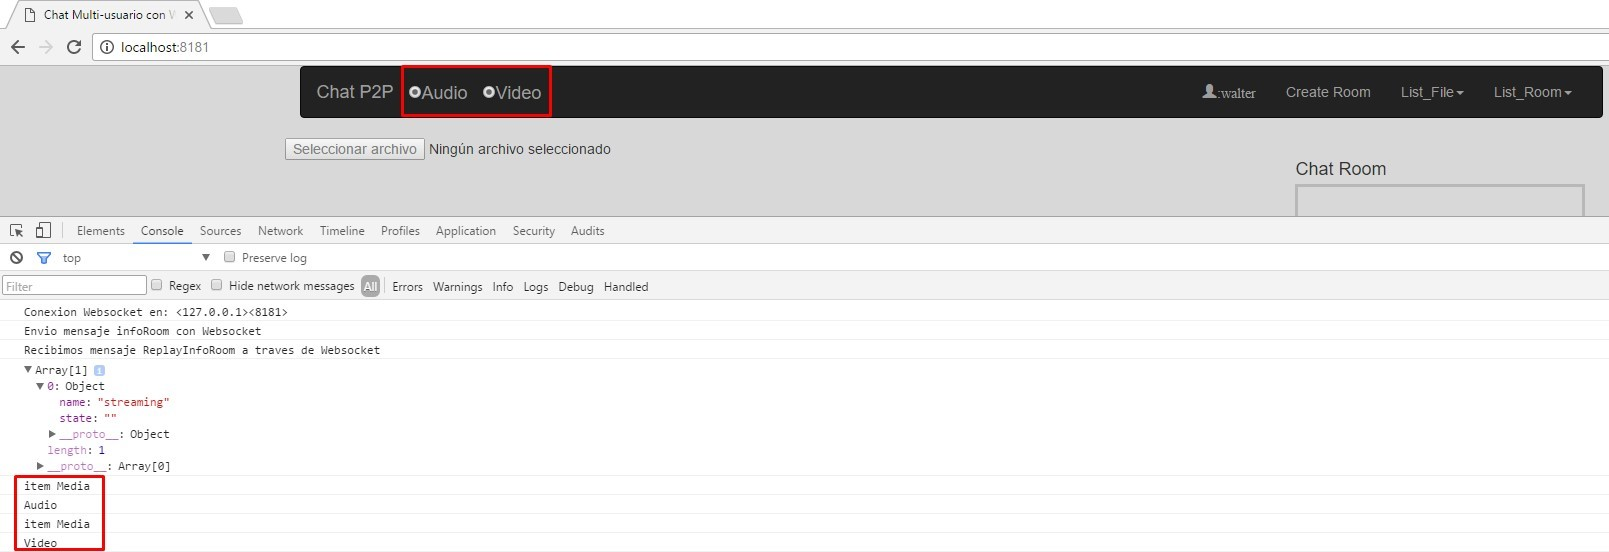
\includegraphics[width=0.8\linewidth]{Figures/SelectItemsClient}
\decoRule
\caption[Petición/Recepción salas.]{Petición/Recepción salas.}
\label{fig:SelectItemsClient}
\end{figure}
\\Una vez los elementos multimedia a compartir han sido seleccionados el usuario puede unirse a una de las salas existentes o crear una nueva sala.
\\Con cualquiera de estas opciones se envía un mensaje \textbf{stablish\_conection} con el nombre del usuario y el de la sala a la que desea conectarse, figura \ref{fig:StablishConnectionClient}.
\begin{lstlisting}[
caption=Envió mensaje inicio conexión.]
 socket.emit('stablish_connection',name,nameRoom);
\end{lstlisting}
Para tratar la respuesta definimos el evento \textbf{CreateStream} con el id de la conexión, figura \ref{fi:StablishConnectionClient}.
\begin{lstlisting}[
caption=Recepción respuesta inicio conexión.]
 socket.on('CreateStream',function(id){
  my_id = id;
 });
\end{lstlisting}
\begin{figure}[!h]
\centering
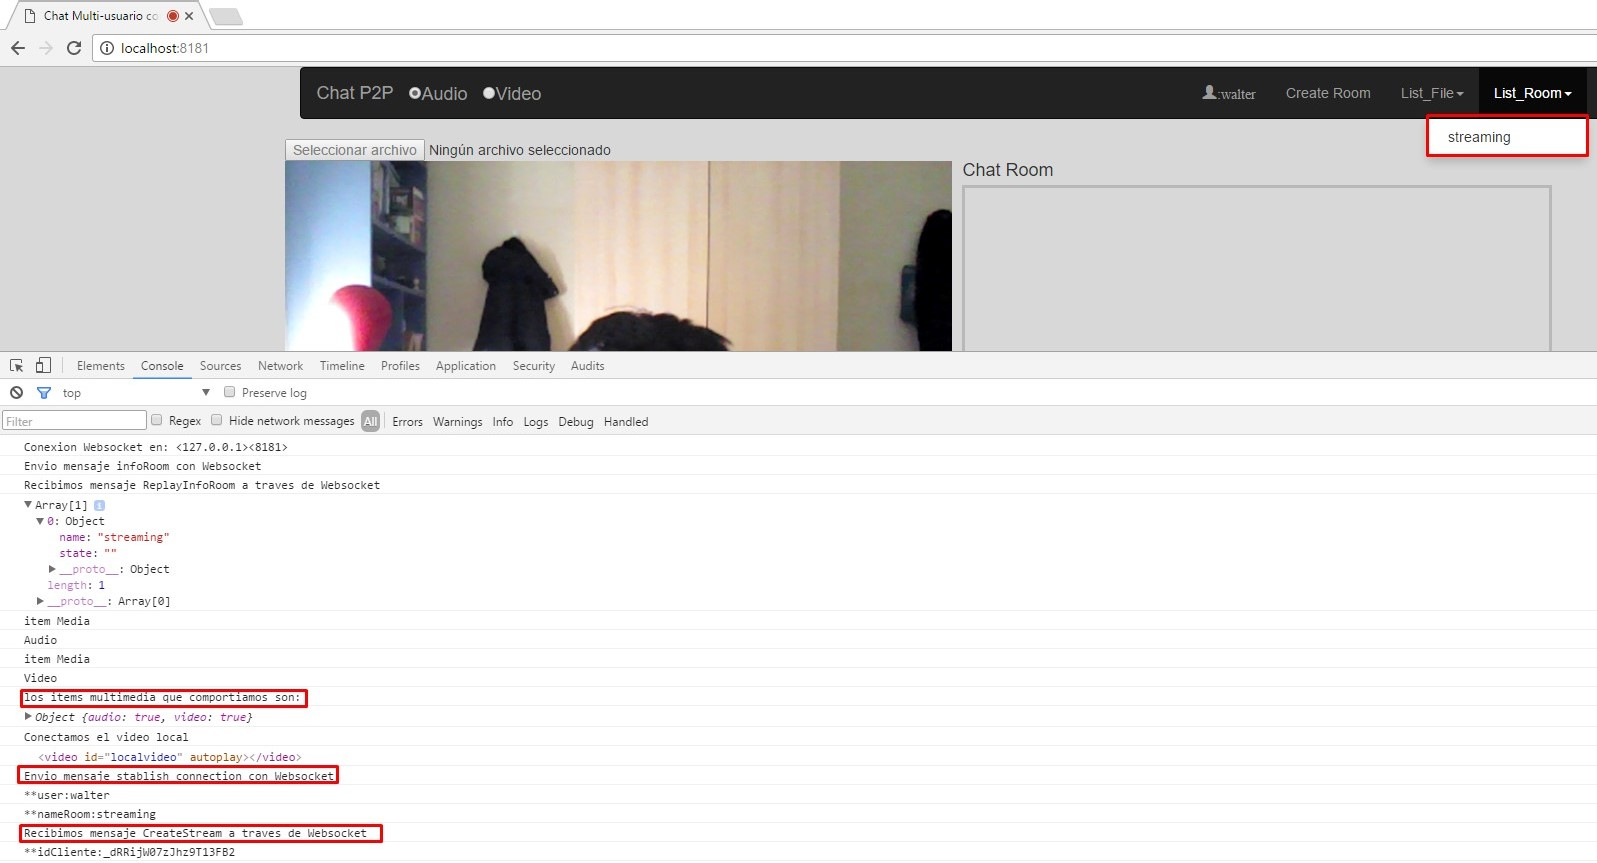
\includegraphics[width=0.8\linewidth]{Figures/StablishConnectionClient}
\decoRule
\caption[Petición/Respuesta establecimiento Conexión.]{Petición/Respuesta establecimiento Conexión.}
\label{fig:StablishConnectionClient}
\end{figure}
Mientras que los demás usuarios recibirán el mensaje 'New\_Joined' con el identificador asociado al usuario que ha solicitado la conexión.
\begin{lstlisting}[
caption=Incluir elementos multimedia remotos l.]
 socket.on('New_Joined',function(id){
  id_newUser = id;
  create_connection(id_newUser);
 });
\end{lstlisting}
A partir de este mensaje empieza el proceso de señalizacion. Este proceso se divide en tres etapas:Offert,Answer y Icecandidate.
%%%%%%%% Cliente offert %%%%%%%%
\subsection*{Offert}
La función \textbf{create\_connection} utiliza el identificador del nuevo cliente e inicia el proceso de oferta.Primero definimos la configuración del  protocolo ICE mediante la variable \textbf{pc\_config} y generamos instancia del objeto \textbf{RTCPeerConnection()} que se almacena en la variable \textbf{pc}.
\begin{lstlisting}[
caption=Instancia RTCPeerConnection.]
 var pc_config = {'iceServers': [{'url': 'stun:stun.l.google.com:19302'}]};
 var pc = new RTCPeerConnection(pc_config,{});
 var num_user = 'user_'+ list_user.length;
 new_remote(num_user);
\end{lstlisting}
Tras esto, es necesario generar una nueva etiqueta de vídeo para tratar el vídeo remoto una vez establecida la conexión.
\begin{lstlisting}[
caption=Creación tag vídeo remoto.]
function new_remote(num_user){
 $('#list_remote').append('<video id='+num_user+'></video');
}
\end{lstlisting}
A continuación, por medio de la variable \textbf{pc} accedemos al método \textbf{addStream()} al que le pasamos el flujo de vídeo local y al evento \textbf{onaddstream} que se encargara de presentar el flujo de vídeo remoto, figura \ref{fig:OfferCliente}.
\begin{lstlisting}[
caption=Vinculamos vídeo local/remoto a RTCPeerConnection.]
 /* video local */
 pc.addStream(streaming);
 /*  video remoto*/
 pc.onaddstream = function(event){
  var video = document.querySelector('#'+num_user);
  video.mozSrcObject = event.stream;
  video.play();
 };
\end{lstlisting}
El siguiente paso es definir el canal de comunicación de datos a través del método \textbf{pc.createDataChannel} al que se le pasa el nombre del canal y definimos los eventos necesarios para manejar los mensajes, figura \ref{fig:DataChannelOffert}.
\begin{lstlisting}[
caption=Instancia de DataChannel.]
 /* canal de datos */
 var sendChannel = pc.createDataChannel("sendDataChannel",{reliable: true})
 /* guardamos el canal */
 list_send.push(sendChannel);	
 /* eventos manejo de datos */
 sendChannel.onopen = ChannelOpen;
 sendChannel.onclose = ChannelClose;
 sendChannel.onmessage = ChannelReceive;
\end{lstlisting}
\begin{figure}[!h]
\centering
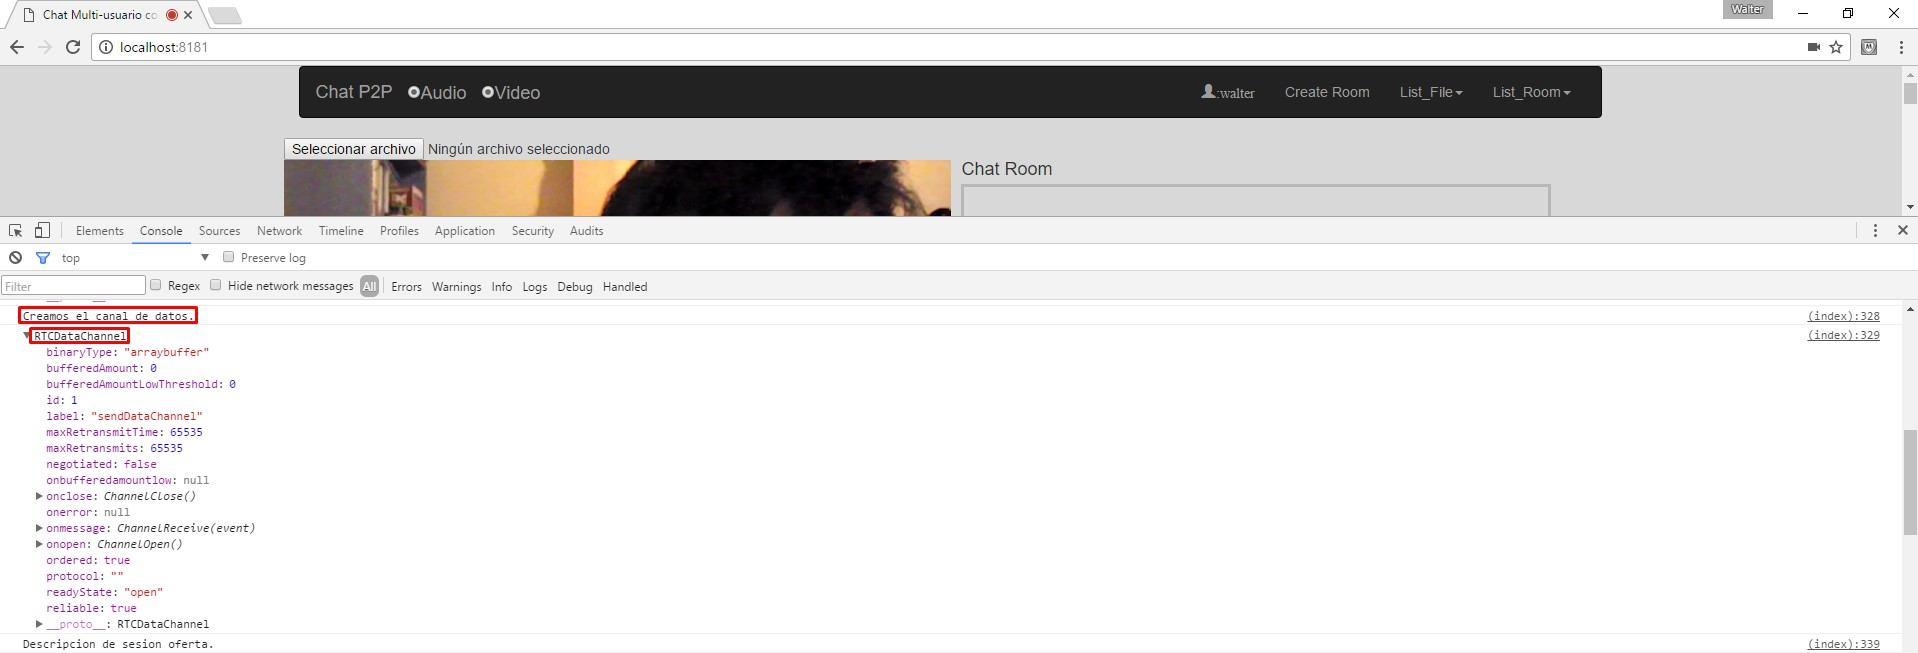
\includegraphics[width=0.8\linewidth]{Figures/DataChannelOffert}
\decoRule
\caption[Creación canal de datos cliente.]{Creación canal de datos cliente.}
\label{fig:DataChannelOffert}
\end{figure}
Finalmente, definimos el método \textbf{pc.createOffer()} en el que guardamos la descripción de sesión local con el método \textbf{pc.setLocalDescription(sessionDescription)} y enviamos un mensaje \textbf{message} donde el cuerpo del mensaje es la oferta generada, figura \ref{fig:OfferCliente}.
\begin{lstlisting}[
caption=Creación de la oferta.]
 pc.createOffer(function(sessionDescription){
  //guardamos esto en nuestra session
  pc.setLocalDescription(sessionDescription);
  //enviamos nuestra descripcion al nuevo usuario
  var message = create_msg(my_id,id_newUser,sessionDescription);
  socket.emit('message',message);
 },function(err){console.log(err);},{});
\end{lstlisting}
\begin{figure}[!h]
\centering
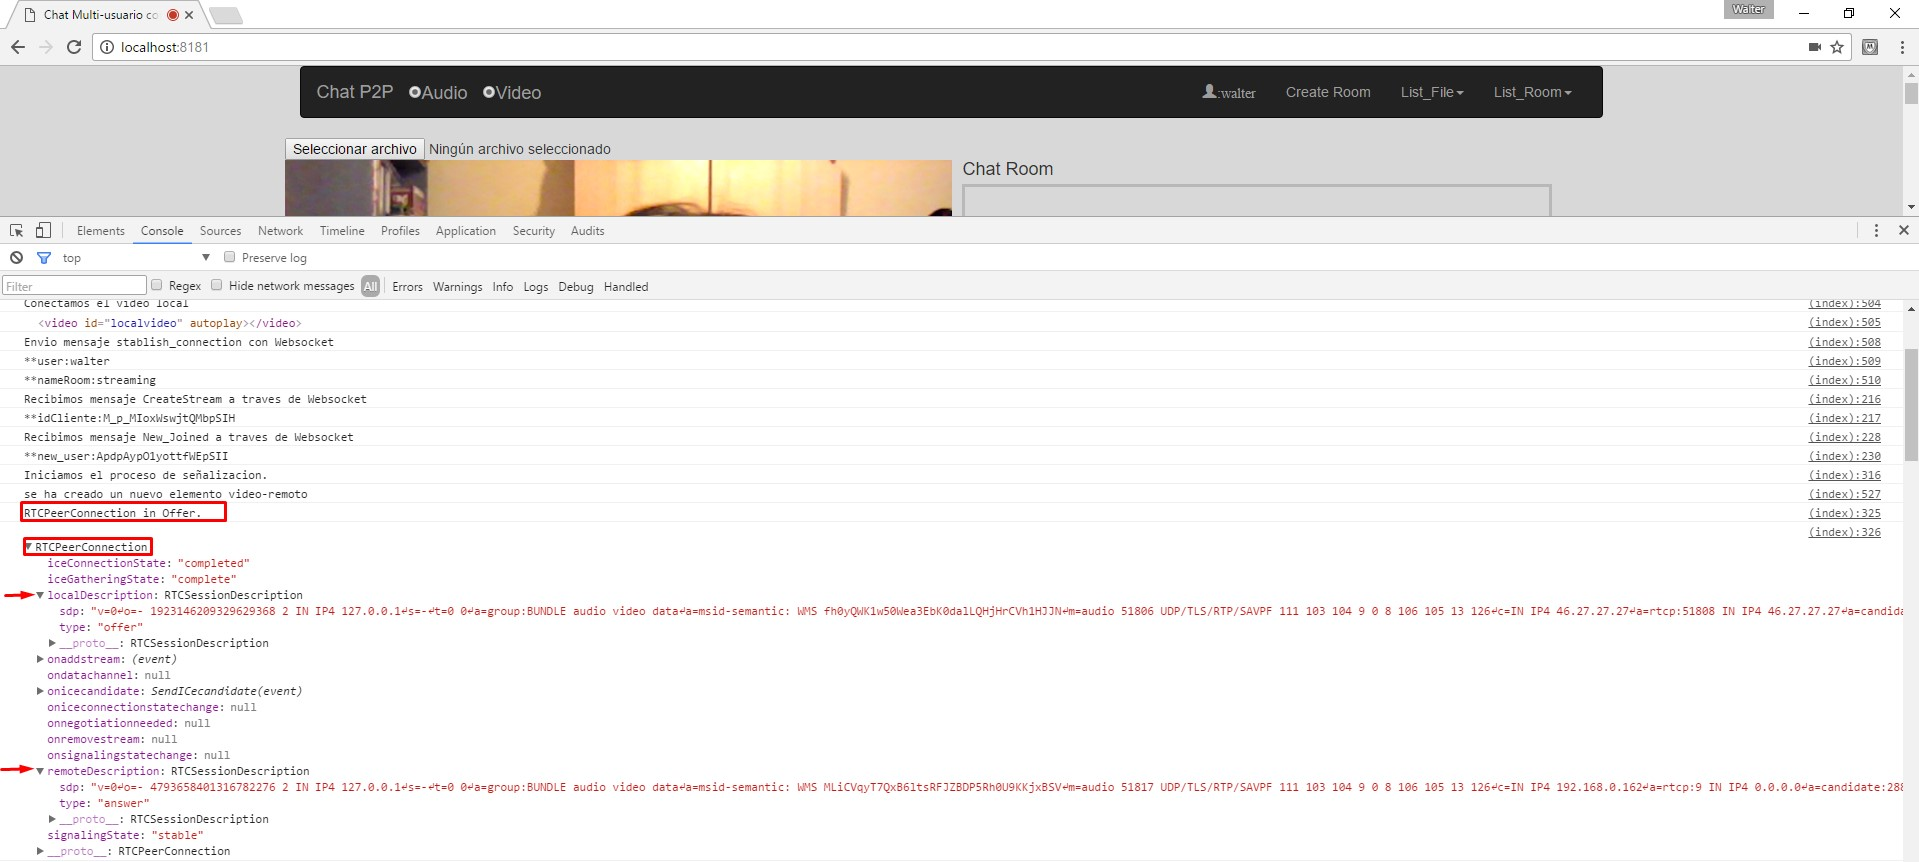
\includegraphics[width=0.8\linewidth]{Figures/OfferCliente}
\decoRule
\caption[Creación oferta cliente.]{Creación oferta cliente.}
\label{fig:OfferCliente}
\end{figure}

%%%%%%%% Cliente Answer %%%%%%%%
\subsection*{Answer}
El cliente que origina la oferta recibe un mensaje de tipo \textbf{message} en el que evaluamos el subtipo de mensaje ya que a través de este tipo de mensaje recibimos los distintos tipos de mensaje de señalizacion.
\\Al principio generamos una instancia de \textbf{RTCPeerconection()} de la misma forma que se realizo en la oferta. A continuación, con la información recibida se genera un nuevo objeto \textbf{RTCSessionDescription} que se guarda como descripción de sesión remota a través del método \textbf{setRemoteDescription()}. 
\begin{lstlisting}[
caption=Guardar descripción de sesión remota.]
 pc.setRemoteDescription(new RTCSessionDescription(message.message));
\end{lstlisting}
El siguiente paso es establecer el canal de comunicación que en este caso tenemos que utilizar el evento \textbf{ondatachannel} ya que solo se puede crear un canal de comunicación entre dos nodos. De igual forma que en la oferta creamos las funciones para los eventos del canal, figura \ref{fig:DataChannelAnswer}. 
\begin{lstlisting}[
caption=Creación de canal de recepción de datos.]
 pc.ondatachannel = function(event){
  list_send.push(event.channel);
  var receiveChannel = event.channel;
  /* evento de recepcion */
  receiveChannel.onmessage = ChannelReceive;
  receiveChannel.onopen = ChannelOpen;
  receiveChannel.onclose = ChannelClose;
 }
\end{lstlisting}
\begin{figure}[!h]
\centering
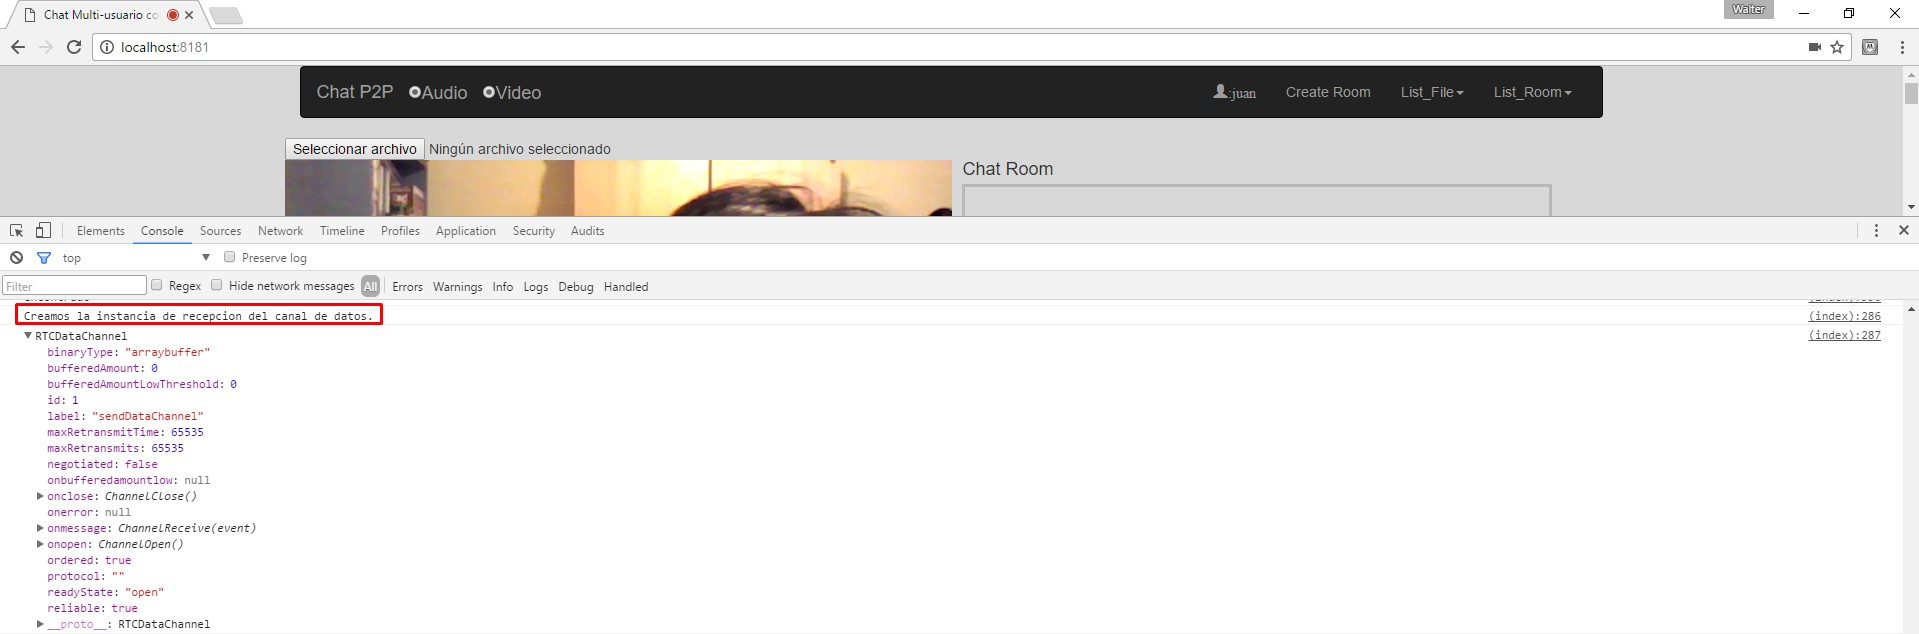
\includegraphics[width=0.8\linewidth]{Figures/DataChannelAnswer}
\decoRule
\caption[Creación canal de recepción datos.]{Creación canal de recepción datos.}
\label{fig:DataChannelAnswer}
\end{figure}
Finalmente, creamos la respuesta a la oferta a través del método \textbf{createAnswer()} dentro del cual guardaremos la información de nuestra propia sesión a través del método \textbf{setLocalDescription} y enviamos un mensaje de tipo \textbf{message} con la información de la sesión local para que el nodo remoto guarde esta información.
\begin{lstlisting}[
caption=Creación de la respuesta.]
 pc.createAnswer(function(sessionDescription){
  pc.setLocalDescription(sessionDescription);
  var msg = create_msg(my_id,message.id_origen,sessionDescription);
  socket.emit('message',msg);
 },function(err){console.log(err);},{});
\end{lstlisting}
\begin{figure}[!h]
\centering
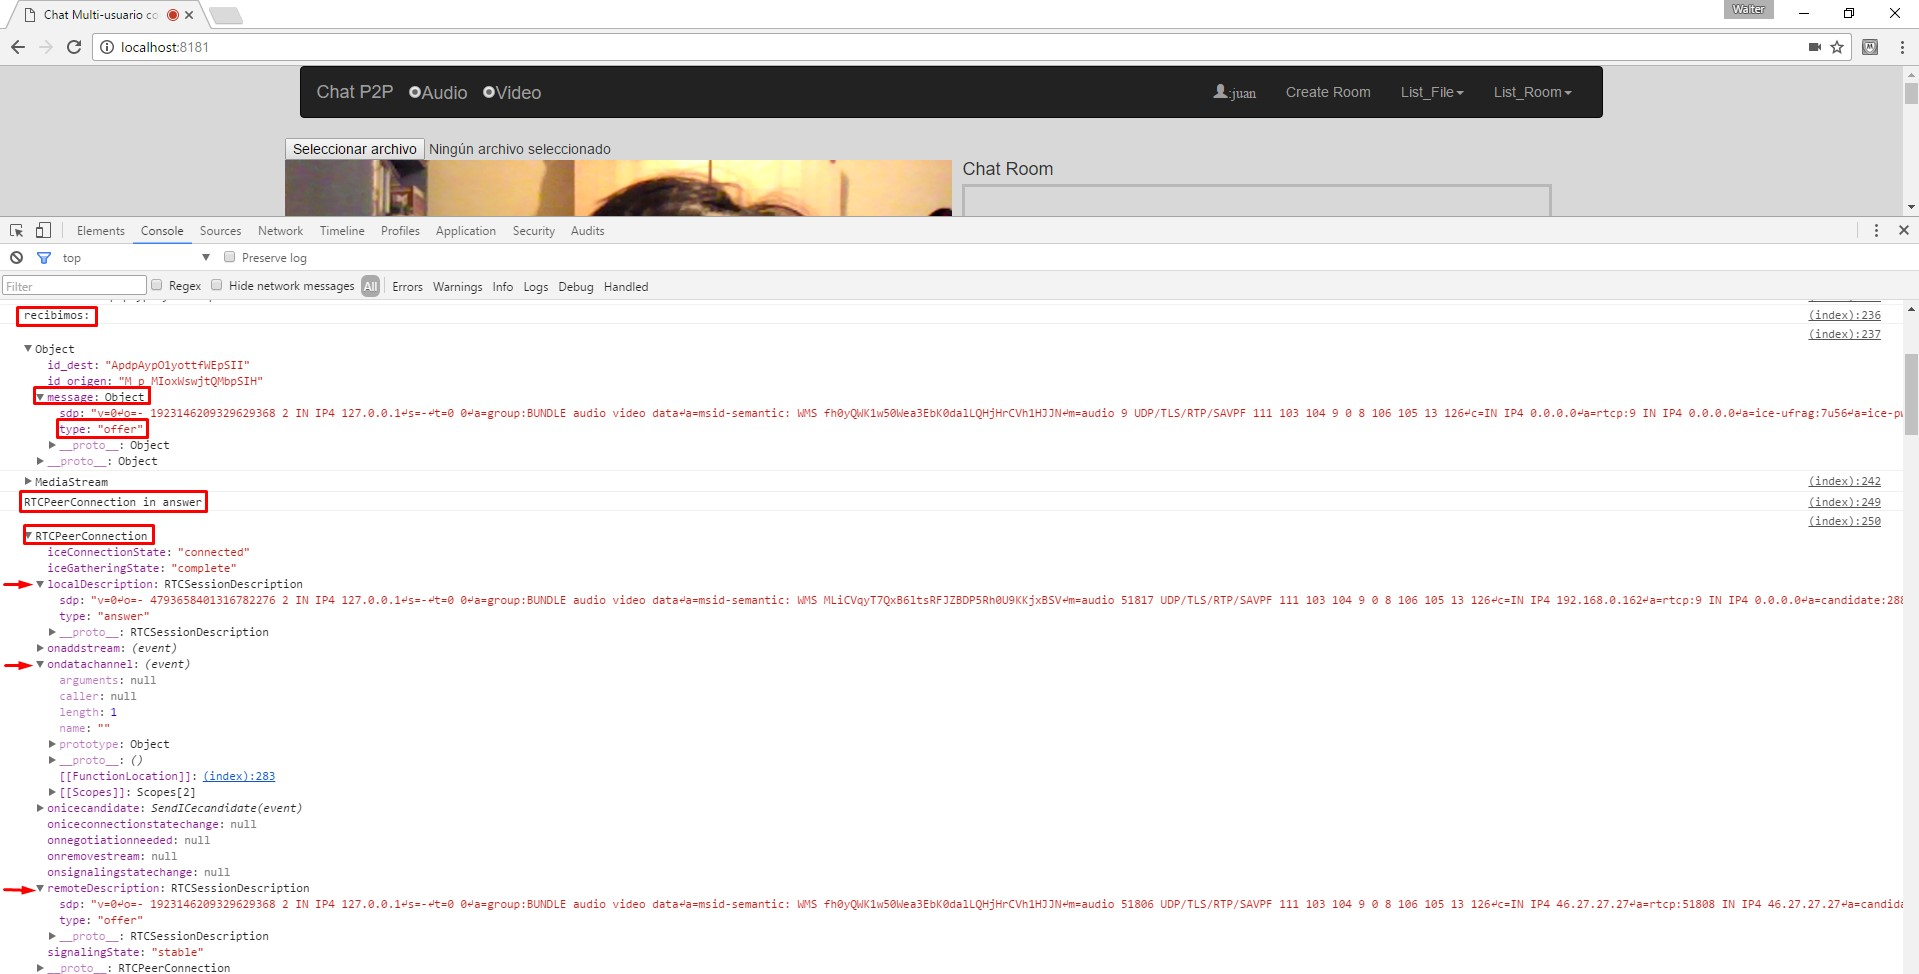
\includegraphics[width=0.8\linewidth]{Figures/AnswerCliente}
\decoRule
\caption[Creación de la respuesta.]{Creación de la respuesta.}
\label{fig:Conexcion_finish}
\end{figure}

%%%%%%%% Cliente IceCandidate %%%%%%%%
\subsection*{Icecandidate}
Tanto el usuario local y como el remoto tras la generación del objeto 'RTCPeerconnectio()' necesitan obtener información de la \textbf{Ip:Puerto} disponibles para la conexión por medio del protocolo ICE.
\\Cuando se encuentra un candidato se ejecuta el evento \textbf{onicecandidate} que compone el mensaje con la información red  y lo envía a través de un mensaje de tipo \textbf{message}.
\begin{lstlisting}[
caption=Envió candidatos.]
 pc.onicecandidate = SendICecandidate;
 ...............
 function SendICecandidate(event){
  if(event.candidate){
   var ice = {type: 'iceCandidate',
    label: event.candidate.sdpMLineIndex,
    id: event.candidate.sdpMid,
    candidate: event.candidate.candidate
   };
   var msg ={id_origen:my_id,id_dest:id_newUser,message:ice}
   socket.emit('message',msg);
  }
}
\end{lstlisting}
Los usuarios que reciben la información anterior generan un objeto \textbf{RTCIceCandidate()} y se llama a la función \textbf{addIcecandidate} que se encarga de buscar dentro de la lista de conexiones la correspondiente y así guardar el objeto creado a través del método \textbf{addIceCandidate}.
\begin{lstlisting}[
caption=Recepción de candidatos.]
 var candidate = new RTCIceCandidate({sdpMLineIndex:message.message.label,
  candidate:message.message.candidate
 });
 addIceCandid(message.id_origen,candidate);
 .............
 function addIceCandid(id,message){
  for(var i=0;i<list_user.length;i++){
   var user = list_user[i];
   if(user.id == id){
    user.peer.addIceCandidate(message);
   }
  }
 }
\end{lstlisting}
Una vez finalizado el proceso de señalizacion la comunicación pasa a ser Peer-to-Peer entre los clientes de una sala, figura \ref{fig:Coneccion_finish}.
\begin{figure}[!h]
\centering
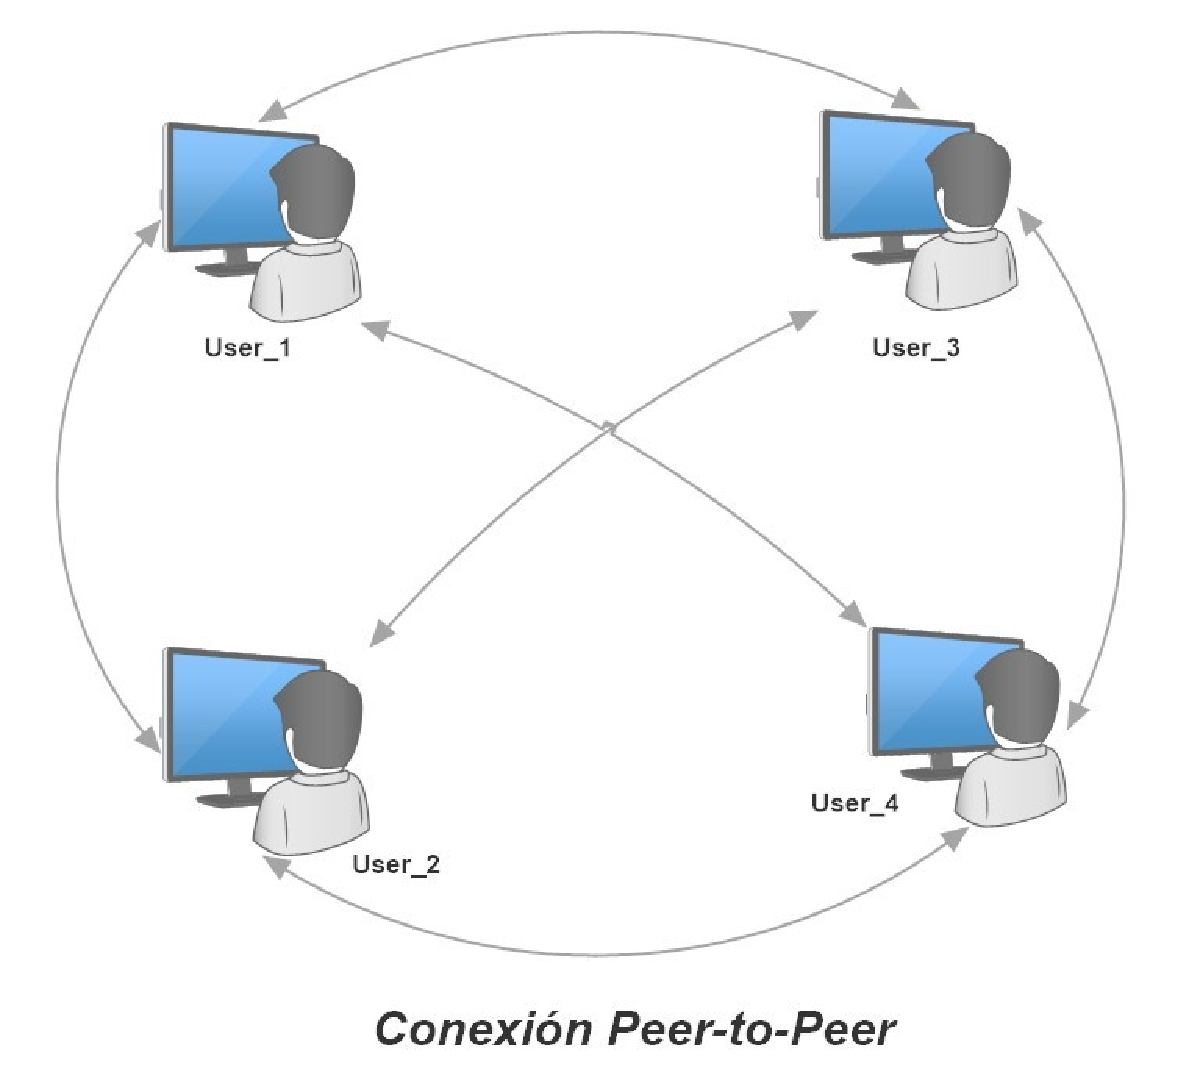
\includegraphics[width=0.5\linewidth]{Figures/Conexcion_finish}
\decoRule
\caption[Conexión Peer-to-Peer final.]{Conexión Peer-to-Peer final.}
\label{fig:Coneccion_finish}
\end{figure}
\subsection*{Envió de cadena de texto}
A través del chat de la sala se puede enviar cadena de caracteres entre los usuarios  mediante la función \textbf{send\_data()}. La función se encarga de obtener los caracteres que el usuario a tecleado y genera un mensaje que contiene el flag \textbf{chat} y el dato obtenido mediante el canal de comunicación, figura \ref{fig:ChatClienteSend}.
\begin{lstlisting}[
caption=Envió datos del chat.]
function send_data(elemento){
  var msg = $(elemento).val();
  var data = JSON.stringify({info:'chat',data:name+':'+msg});
  for(var i=0;i<list_send.length;i++){
   var user = list_send[i];
   user.send(data);
  }
  $(elemento).val('');
}
\end{lstlisting}
\begin{figure}[!h]
\centering
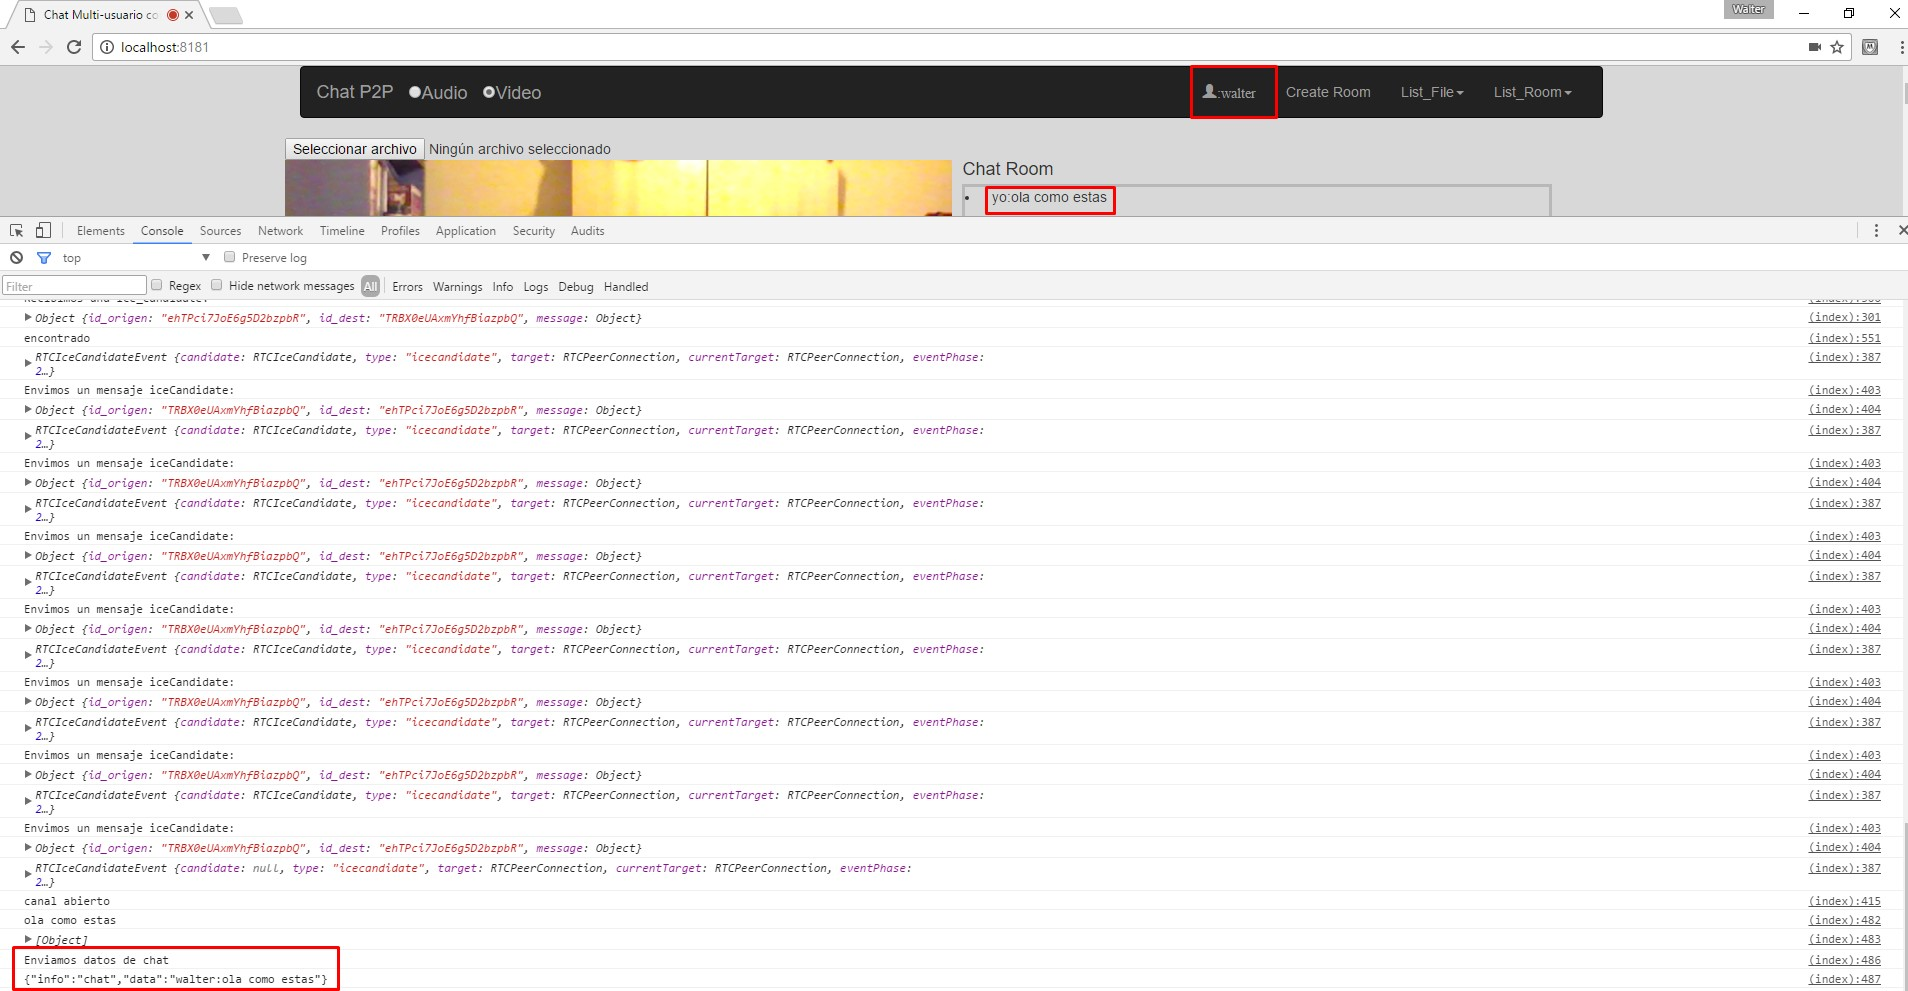
\includegraphics[width=0.8\linewidth]{Figures/ChatClienteSend}
\decoRule
\caption[Envió de caracteres del chat por RTCDataChannel.]{Envió de caracteres del chat por RTCDataChannel.}
\label{fig:ChatClienteSend}
\end{figure}
La recepción por parte de los usuarios se realiza por medio de la función \textbf{WriteChat(\_data)} que se encarga de presentar dentro del chat la información que se ha recibido.
\begin{lstlisting}[
caption=Recepción datos del fichero.]
function WriteChat(_data){
 var line = document.createElement('li');
 var textnode = document.createTextNode(_data.data);
 line.appendChild(textnode);
 $('#texto').append(line);
}
\end{lstlisting}
\subsection*{Envió de ficheros}
Los usuarios disponen de un \textbf{input} de tipo file con el que carga el fichero que desea compartir.Tras seleccionar el fichero se ejecuta la función \textbf{processFiles(file)} para obtener el contenido del fichero a través del objeto \textbf{FileReader()}, figura \ref{fig:fildSendUser}. 
\begin{lstlisting}[
caption=Lectura del fichero.]
 function processFiles(file){
  var files = file[0];
  type = files.type;
  name_fich = files.name;
  var reader = new FileReader();
  reader.onload = function (e) {
   var data_file = reader.result;
   data_encript = arrayBufferToBase64(data_file);
   send_chucky();
  };
  reader.readAsArrayBuffer(files);
 }
\end{lstlisting}
El envió de los datos se realiza por medio de la función \textbf{send\_chucky()} en pequeños fragmentos de longitud fija ya que no sabemos la longitud del archivo y con el fin de no saturar el canal lo enviamos de esta forma.
\\Cada envió por el canal esta formado por el flag \textbf{file} y el fragmento del archivo correspondiente una vez se ha enviado se programa el siguiente envió mediante el evento timer \textbf{setTimeout(sendChuncky,time)}.
\\Al enviar el fragmento final del fichero se añade información adicional del fichero como el nombre y tipo de fichero ya que esta información es necesario para que el usuario receptor pueda reconstruir el fichero, figura \ref{fig:fildSendUser}.
\begin{lstlisting}[
caption=Envió de fragmentos del archivo.]
 function send_chucky(){
  var last = false;
  fin = inicio + size_data;
  if(fin < data_encript.length){
   var data = JSON.stringify({info:'file',data:data_encript.slice(inicio, fin)});
   for(var i=0;i<list_send.length;i++){
    var user = list_send[i];
    user.send(data);
   }
   inicio = fin;
   setTimeout(send_chucky, 100);
  }else{
   last = true;
   var more_info ={type:type,name:name_fich};
   var data = JSON.stringify({info:'file',end:last,data:data_encript.slice(inicio, data_encript.length),more:more_info});
   for(var i=0;i<list_send.length;i++){
    var user = list_send[i];
    user.send(data);
   }
   inicio = 0;
  }
}
\end{lstlisting}
\begin{figure}[!h]
\centering
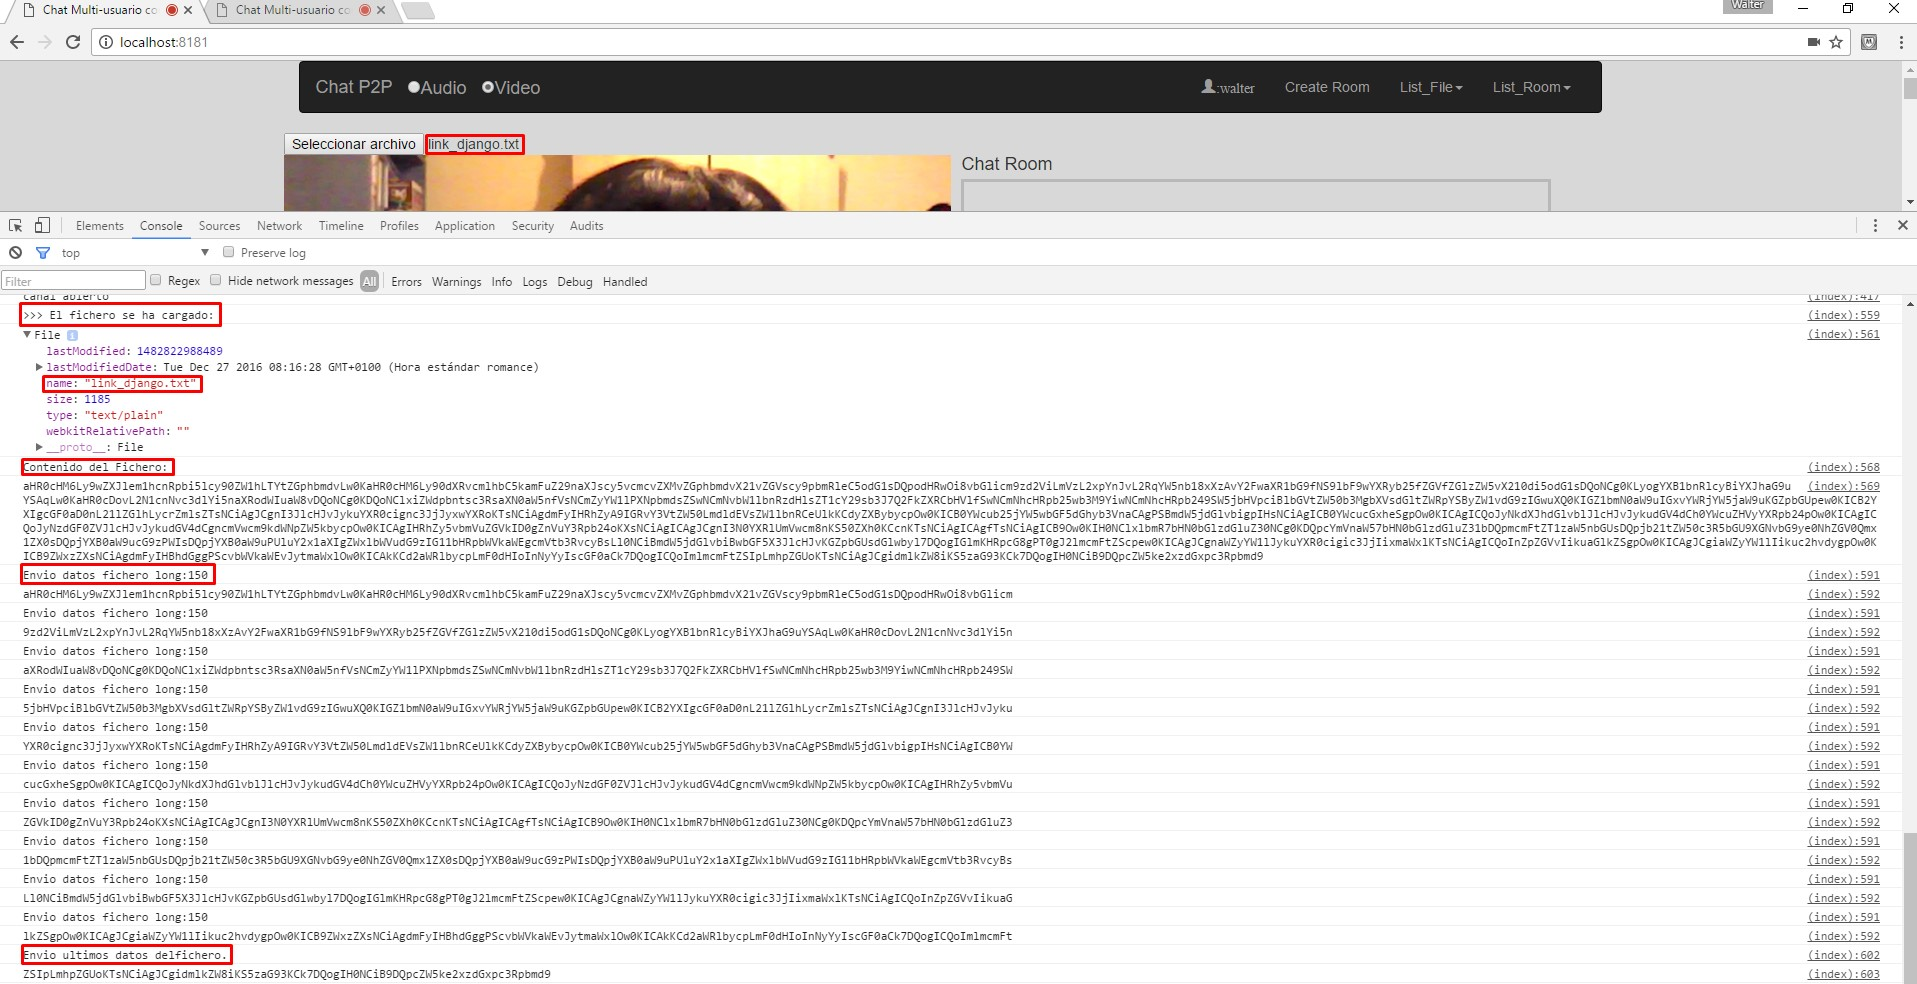
\includegraphics[width=0.8\linewidth]{Figures/filSendUser}
\decoRule
\caption[Envió información del fichero con  RTCDataChannel.]{Envió información del fichero con  RTCDataChannel.}
\label{fig:fildSendUser}
\end{figure}
El usuario receptor ira acumulando cada uno de los fragmentos que reciba hasta obtener el ultimo fragmento mediante la función \textbf{BuildField()}. Al obtener el ultimo fragmento pasamos a generar el documento a través una etiqueta '<a>' donde el atributo href esta formado por el tipo de archivo concadenado a los fragmentos del archivos, figura \ref{fig:FieldReceiveUser}.
\begin{lstlisting}[
caption=Recepción y reconstrucción del fichero .]
 function BuildFile(_data) {
  blob += _data.data;
  if(_data.end != undefined){
   if(_data.more.type == 'text/plain'){
    var link = document.createElement('a');
    link.href = 'data:'+_data.more.type+';base64'+blob;
    link.target = '_blank';
    link.download = _data.more.name;
    var textnode = document.createTextNode(_data.more.name);
    link.appendChild(textnode);
    $("#listFile").append(link);
   }
   blob =',';
  }
 }  
\end{lstlisting}
\begin{figure}[!h]
\centering
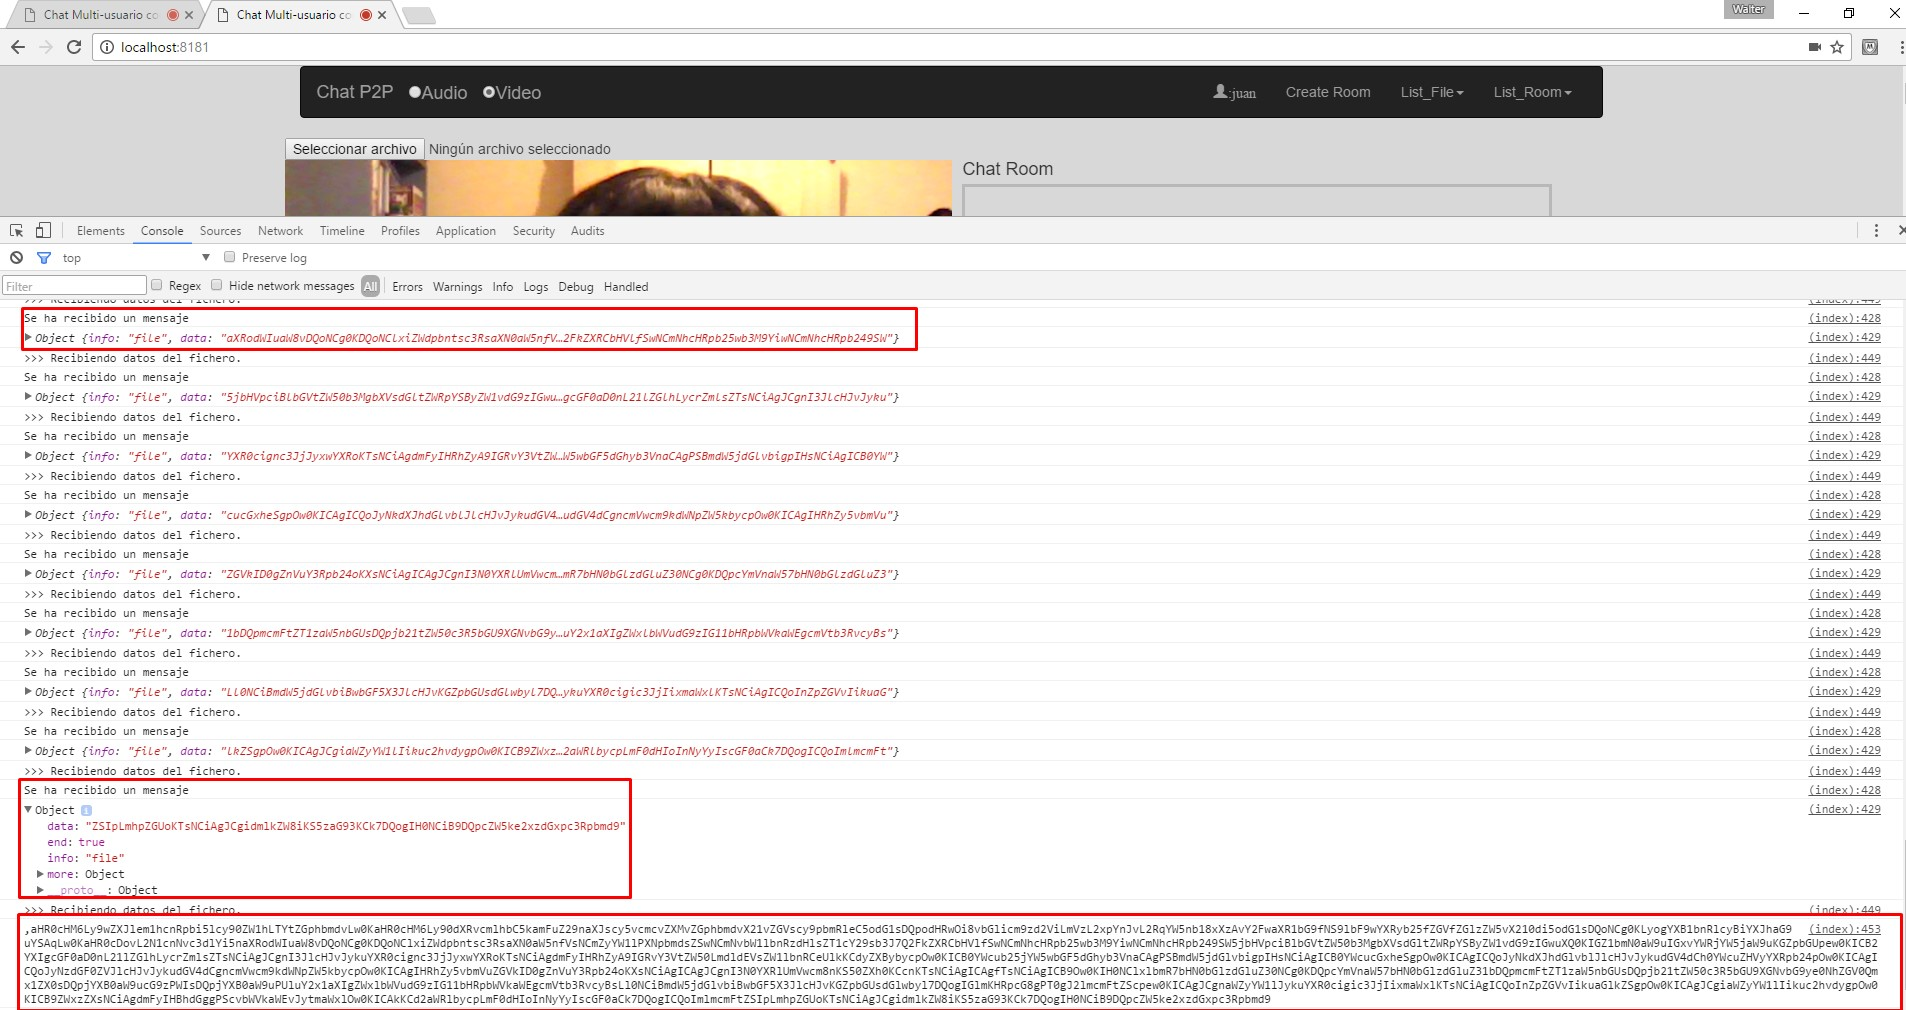
\includegraphics[width=0.8\linewidth]{Figures/filReceiveUser}
\decoRule
\caption[Recepción y reconstrucción del fichero]{Recepción y reconstrucción del fichero.}
\label{fig:FieldReceiveUser}
\end{figure}
\section{Pruebas}
